\chapter{Android jako system operacyjny}

\section{Początki systemu}
Słowo \textit{android} w~czasach obecnych używane jest w~wielu kontekstach. Może odnosić się do humanoidalnego robota, znanego z~literatury science-fiction, ale ostatnio przede wszystkim kojarzone jest z~rynkiem nowoczesnych urządzeń elektronicznych. Są to telefony komórkowe z~dotykowym ekranem (tzw. smartfony), tablety, netbooki, odbiorniki GPS, zegarki, a~także telewizory, lodówki, pralki i~inne urządzenia wykorzystywane w~gospodarstwie domowym. Android to również nazwa firmy, system operacyjny, projekty \textit{Open Source\footnote{Otwarte oprogramowanie (ang. open source movement, dosł. ruch otwartych źródeł) – odłam ruchu wolnego oprogramowania (ang. free software), który proponuje nazwę open source software jako alternatywną dla free software, głównie z~przyczyn praktycznych, a~nie filozoficznych. Obok darmowego udostępniania może ono być sprzedawane i~wykorzystywane w~sposób komercyjny. Sposób osiągania zysków można także ograniczyć do sprzedaży dodatkowych usług, takich jak szkolenia z~obsługi, wsparcie klienta czy dostęp do dodatkowych rozszerzeń, wtyczek, dodatków i~modułów. Możliwe jest też wykorzystanie bezpłatnej wersji open source, jako sposób na zachęcenie do kupna bardziej rozbudowanej wersji dostarczanej na licencji komercyjnej. Źródło: Wikipedia}}, a~nawet społeczność programistów.

Początki systemu Android sięgają roku 2003, kiedy to Andy Rubin, Chris White, Nick Sears oraz Rich Miner założyli w~Kalifornii firmę Android Inc. Głównym celem powstania przedsiębiorstwa była chęć produkcji urządzeń mobilnych, które bazowałyby na danych lokalizacyjnych i~uwzględniały preferencje użytkowników. Jednak zmagająca się z~wymaganiami rynku oraz trudnościami finansowymi firma w~2005 roku została przejęta przez Google Inc., amerykańskie przedsiębiorstwo z~branży internetowej, słynące z~popularnej wyszukiwarki o~tej samej nazwie. Wkrótce potem założono grupę \textit{Open Handset Alliance} (OHA), w~której skład weszły (oprócz Google) takie znane firmy jak HTC, Intel, Motorola, Qualcomm, T-Mobile, Sprint Nextel oraz NVIDIA, a~która stawiała sobie za cel rozwój otwartych standardów dla telefonii mobilnej. Zdecydowanie przyspieszyło to badania nad systemem i~jego rozwój. Pierwsza wersja Androida została przedstawiona światu już w~2007 roku, a~pierwszym telefonem, który korzystał z~tego systemu, był HTC G1.

Dwie premierowe wersje systemu nie miały nazw nadanych zgodnych z~konwencją, do której przywykli użytkownicy z~całego świata. Dopiero począwszy od wersji 1.5, która została wydana 30 kwietnia 2009 roku, oficjalne wersje systemu otrzymywały już nazwy słodkich deserów. Określenia przyznawane są zgodnie z~porządkiem alfabetycznym, więc wersję 1.5 nazwano \textit{Cupcake}.

\section{Udział w~rynku}
Android, jako system operacyjny przeznaczony dla urządzeń mobilnych, według \cite{website:android:stat2} we~wrześniu 2015 roku miał największy udział w~rynku urządzeń na świecie, a~jego wartość przekroczyła 53\%.

\begin{figure}[!htb]
    \centering
    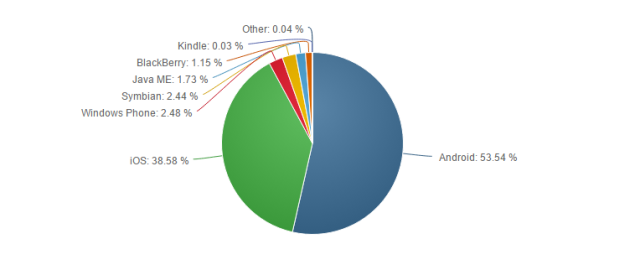
\includegraphics[width=17cm]{imgs/ch2_android_udzial_2.png}
    \caption
{Android – udział w~rynku urządzeń mobilnych na świecie. (Źródło: portal android.com.pl, 09/2015)}
    \label{fig:android_udzial_zagranica}
\end{figure} 

Drugie miejsce na świecie, według tego samego portalu, zajmuje system iOS (38\%), a~trzecie - Windows z~niespełna 3\% udziału. 

W Polsce proporcje są nieco inne. Według \cite{website:android:stat1} także prowadzi Android, którego udział w rynku urządzeń mobilnych wynosi ponad 65\%. Na~drugim miejscu plasuje się system Windows (niespełna 16\%), a~system iOS jest na trzecim miejscu i~zajmuje około 10\% rynku urządzeń mobilnych.

\begin{figure}[!htb]
    \centering
    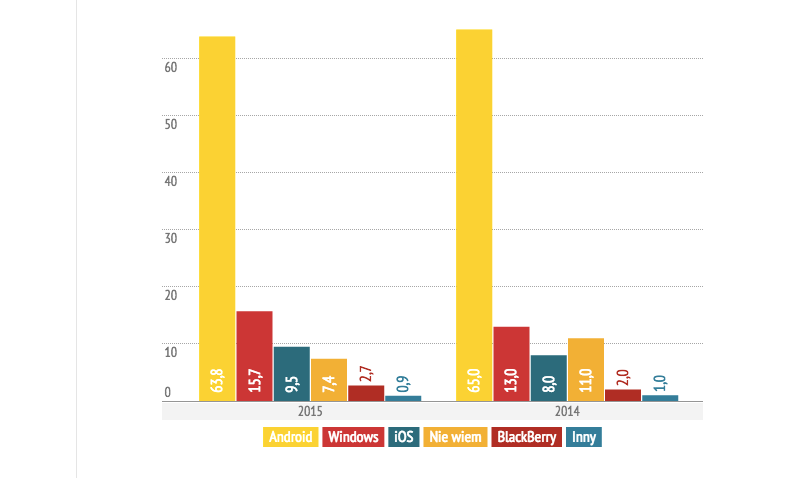
\includegraphics[width=15cm]{imgs/ch2_android_udzial_1.png}
    \caption
{Android – udział w~rynku urządzeń mobilnych w~Polsce. (Źródło: portal AntyWeb.pl, 05/2015)}
    \label{fig:android_udzial_polska}
\end{figure} 

\newpage

\section{Rozwój systemu}
Niezwykle cenną z~punktu widzenia programistów, jest informacja o~udziale poszczególnych wersji Android na urządzeniach posiadanych przez użytkowników. Dzięki niej mogą oni lepiej zoptymalizować swoje aplikacje pod kątem sprzętu. Dane z~września 2015 przedstawia rysunek \ref{fig:android_udzial_wersje}

\begin{figure}[!htb]
    \centering
    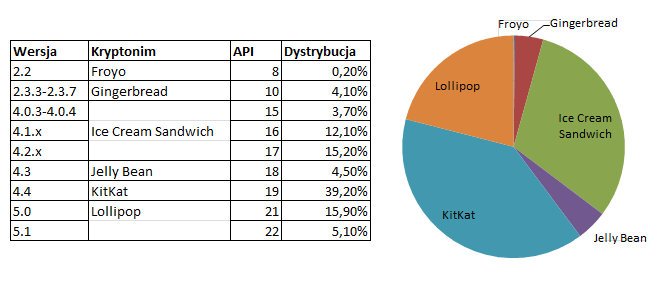
\includegraphics[width=17cm]{imgs/ch2_android_udzial_3pl.png}
    \caption
{Statystyki dotyczące używania poszczególnych wersji systemu Android przez użytkowników (Źródło: portal androidnow.pl, 09/2015). Ostatnio doszła wersja 6.0, ale jej udział na rynku urządzeń w~obecnej chwili jest znikomy.}
    \label{fig:android_udzial_wersje}
\end{figure} 

Z urządzeń, na których instalowany jest Android, większość stanowią smartfony i~tablety. Ale nie tylko. Również urządzenia takie jak \textit{smart-watches}, \textit{smart-TVs}, akcesoria telewizyjne, konsole do gier, piekarniki, pralki, lodówki, satelity wysyłane w~kosmos, a~także najnowsze dziecko firmy Google - Google Glass, wspomagane są tym popularnym systemem operacyjnym. Co więcej, firmy motoryzacyjne zaczynają instalować Androida w~swoich samochodach, rozbudowując w~ten sposób platformę informacyjną i~rozrywkową.

Zgodnie z~manifestem założonej przez Google w~2007 roku grupy \textit{Open Handset Alliance} (OHA), Android został zbudowany z~wykorzystaniem wielu różnych komponentów na licencji \textit{open source}. Zalicza się do nich przede wszystkim jądro Linux, biblioteki programistyczne, kompletne interfejsy użytkownika, aplikacje i~wiele wiele innych. Większość kodu systemu Android jest wydana na licencji \textit{Apache Software License} (ASL, v 2.0). Wyjątkiem jest jądro Linuxa, które wykorzystuje GPLv2 oraz projekt \textit{WebKit} korzystający z~licencji BSD. 

Niestety nie wszystkie części kodu Androida są otwarte dla programistów. Nawet urządzenia z~należącej do Google linii Nexus zawierają komercyjne sterowniki, kodeki, a~nawet całe aplikacje. Jest to duże utrudnienie dla poznających tajniki budowy tego systemu i~próbujących wykorzystać je do pisania własnych aplikacji. Mimo wszystko, wielu programistów, nie pracując dla Google bezpośrednio, zaangażowanych jest w~tworzenie kodu nowych wersji systemu Android. Nie jest to prostym zadaniem, bo z~niezrozumiałych przyczyn firma utrzymuje większość informacji dotyczących rozwoju swojego flagowego produktu w~tajemnicy.

W rozwijanie systemu są zaangażowani jednak nie tylko programiści. Wokół Androida zrzeszeni są również producenci procesorów, kości pamięci RAM, urządzeń, ekranów i~wielu innych części składających się na gotowy produkt.

\section{Programowanie w~systemie w~Android}
Jako system operacyjny dostępny na licencji \textit{Open Source}, Android zrzesza również ogromną społeczność programistów piszących aplikacje poszerzające funkcjonalność urządzeń. W~sierpniu 2014 roku w~internetowym sklepie Google Play (wcześniej Android Market)\footnote{Google Play (dawniej Android Market) – internetowy sklep Google z~aplikacjami, grami, muzyką, książkami, magazynami, filmami i~programami TV. Treści ze sklepu są przeznaczone do korzystania za pomocą urządzeń działających pod kontrolą systemu operacyjnego Android, ale z~niektórych można także korzystać na laptopie czy komputerze stacjonarnym. Źródło: Wikipedia}, dostępnych było ponad 1,3 miliona aplikacji, zarówno płatnych, jak i~darmowych.

Najpopularniejszymi językami programowania, które wykorzystuje się do pisania aplikacji na Androida, są Java i~C++ ze środowiskiem \textit{Android NDK (Native Development Kit)}. o~ile język Java wydawać się może najrozsądniejszym wyborem, o~tyle wielu programistów używa środowiska NDK. Jest to zestaw narzędzi, który pozwala realizować części aplikacji za pomocą kodu macierzystego języków takich jak~C~i~C ++. Zazwyczaj środowisko to wykorzystuje się w~celu pisania programów, które intensywnie wykorzystują CPU, takich jak silniki gier, przetwarzania sygnału czy symulacji fizyki. Jednak deweloperzy muszą wziąć pod uwagę również wady takiego rozwiązania, które mogą nie do końca zbilansować korzyści. Natywny kod Androida na ogół nie powoduje zauważalnej poprawy wydajności. Zwiększa za to znacznie złożoność aplikacji, który to problem i~tak już jest dużym wyzwaniem dla programistów Java. Podsumowując, z~NDK należy korzystać tylko wtedy, jeśli jest to niezbędne dla wytwarzanej aplikacji. Zanim programista zdecyduje się na to rozwiązanie, najpierw powinien sprawdzić, czy androidowe \textit{API\footnote{Interfejs programistyczny aplikacji (ang. Application Programming Interface, API) – sposób, rozumiany jako ściśle określony zestaw reguł i ich opisów, w jaki programy komputerowe komunikują się między sobą. Źródło: Wikipedia}} nie zapewnia już funkcjonalności, jakiej potrzebuje.

Programując aplikacje dla Androida w~języku Java, programiści wykorzystują Android SDK\footnote{SDK - Software Development Kit}. Ten zestaw narzędzi dla programistów, przeznaczony do pisania aplikacji dedykowanych na tę platformę, składa się z~dwóch części: SDK Tools – wymaganej do pisania aplikacji niezależnie od wersji Androida, oraz Platform Tools – czyli narzędzi zmodyfikowanych pod kątem konkretnych wersji systemu. w~skład środowiska programistycznego wchodzi dokumentacja, przykładowe programy, samouczki dla początkujących, biblioteki, emulator oparty na QEMU\footnote{QEMU - szybki emulator napisany przez Fabrice Bellarda.} oraz debugger. SDK dostępne jest zarówno dla Windowsa, jak i~dla Linuxa.

Android SDK ma budowę modularną. Modułami są np. obrazy konkretnych wersji Androida, dodatkowe sterowniki, źródła SDK, czy przykładowe programy. Szczególnie pomocne są obrazy systemu uruchamiane na emulatorze, dzięki którym programiści mogą  testować zachowanie aplikacji na różnych wersjach systemu Android, bez użycia fizycznych urządzeń \cite{website:android:sdk}.

Dużym ułatwieniem dla programistów Javy jest również Android Studio - zintegrowane środowisko programistyczne oparte na IntelliJ IDEA\footnote{IntelliJ IDEA – komercyjne zintegrowane środowisko programistyczne (IDE) dla Javy firmy JetBrains.}. Jego główne zalety to zarządzanie wieloma projektami, współdzielenie plików, możliwość podłączenia do repozytorium, użycie \textit{Gradle} do budowy oprogramowania, możliwość konfiguracji budowy programu w~kilku wariantach dla jednego projektu, możliwość automatycznego uzupełniania kodu oraz wykonywania testów jednostkowych i~integracyjnych bezpośrednio z~narzędzia.

Wspomniany \textit{Gradle} to narzędzie służące do budowania projektów w~Javie. w~przeciwieństwie do jego poprzedników: \textit{Ant}-a i~\textit{Maven}-a, działa w~oparciu o~regułę \textit{„convention over configuration”} polegającą na zminimalizowaniu potrzebnej konfiguracji, poprzez używanie gotowych wartości domyślnych: jeżeli czegoś nie ma w~skrypcie konfiguracyjnym nie znaczy, że nie zostało skonfigurowane i~nie zostanie wykorzystane. Oznacza to tylko, że nie zostały zmienione wartości domyślne.

Java i~C czy C++ to jednak nie wszystkie języki, których można użyć przy programowaniu aplikacji na Androida. Podczas szukania materiałów do tej pracy autor spotkał się z~przykładami aplikacji napisanych w~C\# i Delphi. Stanowią one jednak tak mały udział, że nie będą one brane pod uwagę podczas analizy opisywanego problemu testowalności oprogramowania na ten system operacyjny.


%tutaj przykłady jak użyć poszczególnych konstrukcji
%Przykładowy rysunek \ref{fig:sample_figure}. Prztykładowa tabela %\ref{tab:sample_table}. Przykładowy odnośnik do bibliografi \cite{bib:kowalski_2015}. \textbf{Powodzenia!}


%\begin{figure}[!htb]
%    \centering
%    \includegraphics[width=10cm]{imgs/sample_figure.jpg}
%    \caption{Przykłady rysunek}
%    \label{fig:sample_figure}
%\end{figure} 

%\begin{table}[]
%\centering
%\caption{Przykładowa tabela}
%\label{tab:sample_table}
%\begin{tabular}{|l|l|}
%\hline
%\textbf{Nazwa} & \textbf{Wartość} \\ \hline
%Test           & 1.2              \\ \hline
%Kwiatek        & 5                \\ \hline
%\end{tabular}
%\end{table}